\documentclass[../../tc_tp5_main.tex]{subfiles}

\begin{document}

%capítulo
\chapter{Celda Sallen-Key}

En esta secci\'on, se implementar\'an dos filtros pasabajos haciendo uso de celdas Sallen-Key en cascada. Sobre los mismos, se analizar\'a su respuesta en frecuencia, impedancia de entrada e impedancia de salida, y la sensibilidad de los par\'ametros caracter\'isticos del filtro a desviaciones en los valores de los componentes que lo integran respecto de su valor nominal. \par

Para esto, haremos en primer lugar un an\'alisis te\'orico de las celdas Sallen-Key.


\section{Introducci\'on: la celda Sallen-Key}

La Sallen-Key es una celda que permite realizar un filtro de segundo orden utilizando s\'olo \textit{op amps}, resistencias y capacitores. Si bien normalmente con estos dos tipos de componentes pasivos s\'olo podr\'ian obtenerse polos reales, es decir $Q \leq \nicefrac{1}{2}$, el \textit{feedback} introducido por el operacional permite obtener polos complejos conjugados, y por lo tanto una mayor selectividad. Como en este tipo de celdas existe un \'unico \textit{feedback} positivo, en general la sensibilidad del filtro a la dispersi\'on de los par\'ametros del operacional es menor, y a los valores de los componentes pasivos es mayor, respecto de otro tipo de celdas.\par  

\begin{figure}[H]
	\centering
	\begin{circuitikz}
  	\draw (0,0) node[op amp, yscale=-1] (opamp) {}
  		(opamp.-) -| (-1.5, -1.5) node[left] {$V^-$}
  		to [R = $R_3$, *-]  (-1.5, -3.5) node[ground] {}
  		
  		(-1.5, -1.5) to [R = $R_4$] (1.5, -1.5) 
  		to [short, -*] (1.5, 0) to [short, -o] (2, 0) node[right] {$V_{out}$}
  		(1.5,0) to [short] (opamp.out) 
  		
  		(opamp.+) to [short, -*] (-2.5, 0.5) node[above]{$V^+$}
  		to [generic, l=$Z_3$] (-2.5, -1.5) node[ground]{}
  		
		(-2.5, 0.5) to [generic, l=$Z_2$] (-4.5, 0.5)
		to [generic, l=$Z_1$, *-o] (-6.5, 0.5) node[left]{$V_{in}$}  		
		
		(-4.5, 0.5) to [short, -*] (-4.5, 2) node[above] {$V_f$}
		to [generic, l=$Z_4$] (1.5,2)
		to [short] (1.5,0)
  	;
	\end{circuitikz}
	\caption{Celda Sallen-Key gen\'erica}
\end{figure}

En esta configuraci\'on, las resistencias $R_3$ y $R_4$ son las \'unicas quedeterminan la ganancia de la celda, puesto que forman un circuito no inversor en el camino del \textit{feedback} negativo. Tambi\'en influyen en la ubicaci\'on de los polos y ceros del circuito, junto con las dem\'as resistencias y capacitores que integran la celda.\par

\newpage
Las ecuaciones que describen a este circuito son: 

\begin{equation}
	\left\{
 	\begin{aligned}
 		V_{out} &= A_{vol} \cdot (V^+ - V^-) \\
 		V^+ &= \frac{Z_2}{Z_2+Z_3} V_f  \\
		V^- &= \frac{R_3}{R_3+R_4} V_{out} \\
		\frac{V_{in} - V_f}{Z_1} &= \frac{V_f - V^+}{Z_2} +\frac{V_f - V_{out}}{Z_4} 
	\end{aligned}
	\right.
 \end{equation}
 
De esta \'ultima ecuaci\'on y expresando $V_f$ como funci\'on de $V^+$ se puede obtener que:

\begin{equation}
	V^+ = \left[ \left(1 + \frac{Z_3}{Z_2}\right) \cdot \left( \frac{1}{Z_1} + \frac{1}{Z_2} + \frac{1}{Z_4}\right) - \frac{1}{Z_2}\right] \cdot
			\left( \frac{V_{in}}{Z_1} + \frac{V_{out}}{Z_4}\right) = \frac{d}{Z_1} V_{in} + \frac{\gamma}{Z_4} V_{out}
\end{equation}

Por simplicidad, se efectu\'o la sustituci\'on $\gamma = \left(1 + \frac{Z_3}{Z_2}\right) \cdot \left( \frac{1}{Z_1} + \frac{1}{Z_2} + \frac{1}{Z_4}\right) - \frac{1}{Z_2}$.
Si llamamos adem\'as $K = 1 + \nicefrac{R_4}{R_3}$ a la ganancia del no inversor, esto se puede expresar mediante el siguiente diagrama de flujo de se\~nal: \par

\begin{figure}[H]
	\centering
	\includegraphics[scale=0.5]{imagenes/tc_tp1_ej1_df_1.png}
	
	\caption{Diagrama de flujo de se\~nal del circuito}
\end{figure}

Sucesivas simplificaciones permiten llevar el diagrama anterior a una forma que nos permita ver claramente los \textit{loops} de \textit{feedback} del circuito

\begin{figure}[H]
	\centering
	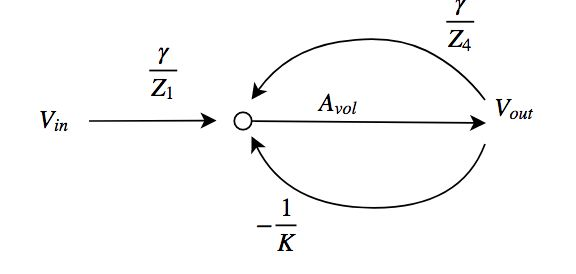
\includegraphics[scale=0.5]{imagenes/tc_tp1_ej1_df_2.jpg}\\
	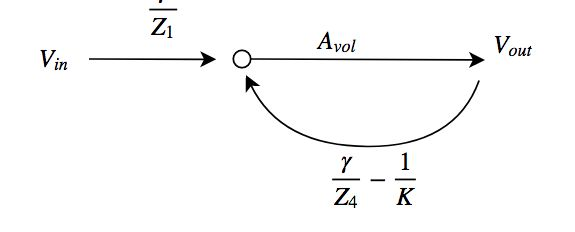
\includegraphics[scale=0.5]{imagenes/tc_tp1_ej1_df_3.jpg}	
	\caption{Simplificaciones del diagrama de flujo de se\~nal}
	\label{fig:1-flujo-de-senal}
\end{figure}

Partiendo de la figura \ref{fig:1-flujo-de-senal}, se puede obtener trivialmente la transferencia como:

\begin{equation}
	\frac{V_{out}}{V_{in}} = \frac{\gamma}{Z_1} \cdot \left( \frac{A_{vol}}{1 + A_{vol} \cdot \left( \frac{\gamma}{Z_4} - \frac{1}{K} \right)} \right)
	\label{eq:1-tf-sk-generica-avol}
\end{equation}

Si consideramos el caso ideal $A_{vol} \to \infty$, volviendo a reemplazar por el valor original de $\gamma$ obtenemos que:

\begin{equation}
	\frac{V_{out}}{V_{in}} = \frac{K}{ \frac{Z_1 Z_2}{Z_3 Z_4} + \frac{Z_1}{Z_3} + \frac{Z_2}{Z_3} + \frac{Z_1 \cdot (1-K)}{Z_4} + 1} 
	\label{eq:1-tf-sk-generica}
\end{equation}

En el caso particular de la celda Sallen-Key pasabajos, las sustituciones que se realizan son:

\begin{equation*}
	\left\{
 	\begin{aligned}
		Z_1 &=  R_1 & Z_3 &= \frac{1}{sC_2}\\
		Z_2 &= R_2 & Z_4 &= \frac{1}{sC_1}\\
	\end{aligned}
	\right.
 \end{equation*}


\begin{figure}[H]
	\centering
	\begin{circuitikz}
  	\draw (0,0) node[op amp, yscale=-1] (opamp) {}
  		(opamp.-) -| (-1.5, -1.5) 
  		to [R = $R_3$, *-]  (-1.5, -3.5) node[ground] {}
  		
  		(-1.5, -1.5) to [R = $R_4$] (1.5, -1.5) 
  		to [short, -*] (1.5, 0) to [short, -o] (2, 0) node[right] {$V_{out}$}
  		(1.5,0) to [short] (opamp.out) 	
  		
  		(opamp.+) to [short, -*] (-2.5, 0.5)
  		to [C, l_=$C_2$] (-2.5, -1.5) node[ground]{}
  		
		(-2.5, 0.5) to [R, l_=$R_2$] (-4.5, 0.5)
		to [R, l_=$R_1$, *-o] (-6.5, 0.5) node[left]{$V_{in}$}  		
		
		(-4.5, 0.5) to [short] (-4.5, 2)
		to [C, l=$C_1$] (1.5,2)
		to [short] (1.5,0)
  	;
	\end{circuitikz}
	\caption{Celda Sallen-Key pasabajos}
\end{figure}

 
Reemplazando en la ecuaci\'on \ref{eq:1-tf-sk-generica}, se obtiene que:

\begin{equation}
	\frac{V_{out}}{V_{in}} = \frac{K}{ s^2 \cdot R_1 R_2 C_1 C_2 + s \cdot \left[ R_1 (1-K) C_1 + (R_1 + R_2) C_2 \right] + 1}
\end{equation}

Efectivamente, esta ecuaci\'on corresponde a un filtro pasabajos de segundo orden, cuyos par\'ametros caracter\'isticos son:

\begin{equation}
	\left\{
 	\begin{aligned}
		f_0 &= \frac{1}{2\pi} \cdot \sqrt{\frac{1}{ R_1 R_2 C_1 C_2 }}\\
		Q &= \frac{\sqrt{ R_1 R_2 C_1 C_2 }}{  (R_1 (1-K) C_1 + (R_1 + R_2) C_2 }\\	
		G &= 1 + \frac{R_4}{R_3} 	
	\end{aligned}
	\right.
 \end{equation}
 
Como se ver\'a m\'as adelante, los dos filtros implementados con estas celdas tienen ganancia unitaria. Si bien podr\'ian utilizarse ganancias distintas de 1 en cada etapa, y si fuese necesario compensarlo con una etapa inversora o no inversora, por simplicidad s\'olo se considerar\'a el caso K = 1. Un posible problema de utilizar este criterio es que obtener un valor elevado de Q puede tornarse m\'as dif\'icil, o simplemente imposible, dadas las restricciones pr\'acticas a la hora de determinar los valores de los componentes. Sin embargo cabe destacar tambi\'en que si $K>1$, se debe prestar particular atenci\'on a no llegar a valores negativos para el coeficiente lineal del denominador de la transferencia, puesto que esto har\'ia que el sistema pierda su estabilidad, y por lo tanto as\'i nos desentendemos de este problema. \par

Para obtener ganancia unitaria, entonces, se reemplaza la resistencia $R_4$ por un cable y se deja un circuito abierto donde estar\'ia $R_3$, de forma tal que $G = 1 + \frac{R_4}{R_3} = 1$.
 
\begin{figure}[H]
	\centering
	\begin{circuitikz}
  	\draw (0,0) node[op amp, yscale=-1] (opamp) {}
  		(opamp.-) -| (-1.5, -1.5) 
		 to [short] (1.5, -1.5) 
  		to [short, -*] (1.5, 0) to [short, -o] (2, 0) node[right] {$V_{out}$}
  		(1.5,0) to [short] (opamp.out) 

  		(opamp.+) to [short, -*] (-2.5, 0.5)
  		to [C, l_=$C_2$] (-2.5, -1.5) node[ground]{}
  		
		(-2.5, 0.5) to [R, l_=$R_2$] (-4.5, 0.5)
		to [R, l_=$R_1$, *-o] (-6.5, 0.5) node[left]{$V_{in}$}  		
		
		(-4.5, 0.5) to [short] (-4.5, 2)
		to [C, l=$C_1$] (1.5,2)
		to [short] (1.5,0)
  	;
	\end{circuitikz}
	\caption{Celda Sallen-Key pasabajos con ganancia unitaria}
	\label{fig:1-celda}
\end{figure}

Con esta configuraci\'on, las expresiones finales de $Q$ y $f_0$ son:

\begin{equation}
	\left\{
 	\begin{aligned}
		f_0 &= \frac{1}{2\pi} \cdot \sqrt{\frac{1}{ R_1 R_2 C_1 C_2 }}\\
		Q &= \frac{\sqrt{ R_1 R_2 C_1 }}{  (R_1 + R_2) \sqrt{C_2} }\\	
		G &= 1 
	\end{aligned}
	\right.
	\label{eq:f0-q}
 \end{equation}

Por \'ultimo, queda analizar la impedancia de entrada y de salida de este circuito, de forma tal que se pueda tener criterio para realizar la conexi\'on en cascada de distintas etapas que lo utilicen. A grandes rasgos, se puede observar que la impedancia de salida no es sino la del operacional que se utilice, que si se lo considera ideal es 0. Por lo tanto, para concatenar esta celda con otra del mismo tipo s\'olo se requiere que la impedancia de entrada no sea comparable con la salida de un \textit{opamp}. Como hay una resistencia en serie a la entrada del circuito, esta establecer\'a un valor m\'inimo para la impedancia de entrada: mientras que esta resistencia sea de cientos de $\Omega$ o m\'as, no deber\'ia observarse que las etapas se carguen entre s\'i.\par 



\subsection{An\'alisis de sensibilidades} 

Antes de determinar los valores de los componentes que se utilizar\'an para cada filtro, estudiaremos a qu\'e componentes es m\'as sensible cada par\'ametro del circuito. A partir de las expresiones obtenidas en \ref{eq:f0-q}, utilizando la f\'ormula $S_x^y = \frac{x}{y} \cdot \frac{\partial y}{\partial x}$, se calcularon las sensibilidades relativas de $f_0$ y $Q$ a peque\~nas variaciones en los valores de los componentes que las integran.

\begin{table}[H]
	\centering
	\begin{tabular}{|c||c|c|c|c|}
	\hline
      	& $R_1$                                       & $R_2$                                     & $C_1$              & $C_2$              \\ \hline \hline
	$f_0$ & $-\nicefrac{1}{2}$                          & $-\nicefrac{1}{2}$                        & $-\nicefrac{1}{2}$ & $-\nicefrac{1}{2}$ \\ \hline
	$Q$   & $ - \frac{R_1 - R_2}{2 \cdot (R_1 + R_2)} $ & $ \frac{R_1 - R_2}{2 \cdot (R_1 + R_2)} $ & $\nicefrac{1}{2}$ & $\nicefrac{1}{2}$  \\ \hline
	\end{tabular}
	
	\caption{Sensibilidades de $f_0$ y $Q$ a los valores de los componentes}
\end{table}

Seg\'un estos resultados, la frecuencia del polo de una celda Sallen-Key de ganancia unitaria tiene la misma sensibilidad respecto de cada componente. En cuanto al factor de calidad, por otro lado, la sensibilidad a los capacitores es siempre $\nicefrac{1}{2}$, pero a las resistencias depende de los valores de las mismas. Al igual que ocurr\'ia antes, $Q$ ser\'a siempre igual de sensible a ambas resistencias, aunque en este caso con signo opuesto, pero ahora si $R_1 = R_2$, esta sensibilidad es 0. Cuanto m\'as cercanos sean los valores de $R_1$ y $R_2$ entre s\'i, y m\'as grandes sean estos valores, menos sensible ser\'a $Q$ a estos par\'ametros. \par 

Por lo tanto, se tomar\'a el criterio de trabajar con resistencias iguales o cercanas entre s\'i, y siempre en el orden de los $k\Omega$. De esta manera, la sensibilidad de $Q$ a las resistencias no deber\'ia ser demasiado elevada. Por ejemplo, si se tomase en una celda $R_1 = 1k\Omega$ y $R_3 = 3k\Omega$, se tendr\'ia que $S_R^Q = \pm 0.5$, es decir que ser\'ia id\'entica a $S_C^Q$.\par 

Por otro lado, como todas las sensibilidades de $f_0$ son $-0.5$ y no se cont\'o con la posibilidad de utilizar capacitores de tolerancias inferiores al $10\%$ para todos los valores, sabemos a priori que cada capacitor podr\'ia introducir un cambio de $-0.5 \cdot(\pm 10\%) = \mp5\%$ en el valor de $f_0$. Como hay dos capacitores por celda, esta dispersi\'on asciende a $10\%$. Por lo tanto, se determin\'o utilizar resistencias de tolerancia $1\%$, ya que de usar $5\%$ los cambios en los par\'ametros caracter\'isticos del circuito podr\'ian ascender al $15\%$, mientras que de esta manera se logra limitar este valor a $11\%$.


\section{Filtro 1: Legendre para alta se\~nal}

En primer lugar, se busca implementar un filtro pasabajos que cumpla la siguiente plantilla:

\begin{table}[H]
	\centering
	\begin{tabular}{|c|c|c|c|}
	\hline	
	Orden & $f_p$   & $A_p$ & $\abs{Z_{in}(f)}$           \\ \hline
	5     & $33kHz$ & $3dB$ & $\geq 50k\Omega\, \forall f$ \\ \hline
	\end{tabular}
	\caption{Plantilla del filtro pasabajos con Legendre}
\end{table}

Como no se tiene restricciones de $A_a$, se determin\'o utilizar $A_p' = 1dB$ a la hora de calcular la transferencia, de forma tal que la tolerancia de los valores de los componentes no provoque que no se cumpla la plantilla.\par

Habiendo obtenido la funci\'on transferencia de este filtro mediante la aproximaci\'on de Legendre, poniendo adem\'as la condici\'on de que todas las etapas deben tener ganancia unitaria, las etapas que se deben dise\~nar son las siguientes:

\begin{table}[H]
	\centering
	\begin{tabular}{|c||c|c|c|}
	\hline
	Etapa & Orden & $f_0\, (kHz)$ & Q    \\ \hline \hline
	1     & 1     & 29.5          & -    \\ \hline
	2     & 2     & 34.2          & 0.72 \\ \hline
	3     & 2     & 40.3          & 2.23 \\ \hline
	\end{tabular}
	\caption{Etapas del filtro 1}
\end{table}

El criterio que se tom\'o para ordenar las etapas fue seg\'un el $Q$: como se debe trabajar en altas se\~nales, se pusieron primero las etapas que menores sobrepicos presentaban, es decir en primer lugar la etapa de orden 1 (que no presenta sobre pico en absoluto) y luego las de orden 2 ordenadas por $Q$ creciente. De esta manera, cuando la se\~nal se amplifica debido al sobrepico ya no es la de entrada (de amplitud alta), sino una que ya pas\'o por al menos una etapa de atenuaci\'on, y por lo tanto el rango din\'amico del circuito mejora respecto de otras configuraciones. \par

Como no se puede implementar una etapa de primer orden con una celda Sallen-Key, se utiliz\'o un circuito integrador compensado.

\begin{figure} [H]
	\centering
	\begin{circuitikz}
	
  		\draw (0,0) node[op amp] (opamp) {}
  		(opamp.-) to [R, l_=$R_1$, *-o] ($(opamp.-)-(2,0)$) node[left]{$V_{in}$}
  		(opamp.-) |- ($(opamp.-)+(0.2,1)$) to[C=$C_1$] ($(opamp.-)+(2.2,1)$) -|
  		(opamp.out) to[short,*-] ($(opamp.out)+(.5,0)$) node [right] {$V_{out}$} node [ocirc] {} 
  
  		 ($(opamp.-)+(0.2,1)$)  
  		 to [short, *-] ($(opamp.-)+(0.2,3)$) 
		to [R,  l_=$R_2$, ] ($(opamp.-)+(2.2,3)$) 
 		to  [short, -*]($(opamp.-)+(2.2,1)$)
 		
 		(opamp.+) to[short] ($(opamp.+) - (0,.5)$) node[ground] {}
  		;\end{circuitikz}
	\caption{Circuito integrador compensado}
\end{figure}

La transferencia de este circuito, considerando al operacionales como ideal, es:

\begin{equation}
	H(s) = - \frac{R_2}{R_1} \cdot \left(\frac{1}{s \cdot R_1 C_1 + 1}\right)
\end{equation}

Por lo tanto en esta etapa se debe cumplir que:

\begin{equation}
	\left\{
 	\begin{aligned}
 		f_0 &= \frac{1}{2\pi \cdot R_1 C_1} \\
 		\frac{R_2}{R_1} &= 1
	\end{aligned}
	\right.
	\label{eq:int-comp}
\end{equation}

Los valores de los componentes se calcularon, pues, a partir de las f\'ormulas \ref{eq:f0-q} y \ref{eq:int-comp}. Considerando adem\'as que los capacitores deb\'ian estar en el orden de los nanofaradios, se determinaron los siguientes valores:

\begin{table}[H]
	\centering
	\begin{tabular}{|c||c|c|c|c|}
	\hline
	Etapa & $R_1\, (k\Omega)$ & $R_2\, (k\Omega)$ & $C_1\, (nF)$ & $C_2\, (nF)$ \\ \hline \hline
	1     & 1                 & 1                 & 5.4          & -            \\ \hline
	2     & 3.5               & 2.2               & 3            & 1.5          \\ \hline
	3     & 1.1               & 1.1               & 16.3         & .820         \\ \hline
	\end{tabular}
	\caption{Valores de los componentes del filtro 1}
\end{table}

Si bien estos valores requieren realizar una cantidad considerable de combinaciones serie y paralelo de componentes, los mismos pueden obtenerse con un error inferior al 1\% para todos los casos.\par 

En este punto, el circuito propuesto no estar\'ia cumpliendo la condici\'on de tener impedancia de entrada mayor a $50k\Omega$: puesto que la primera etapa es el integrador, la impedancia de este circuito es constante $R_1 = 1k\Omega$ (considerando los \textit{op amps} como ideales). Si se corrigiese esto con $R_1 = R_2 = 50k\Omega$, se obtendr\'ia un valor de $C_1 = 108pF$. Consideramos que este valor es demasiado peque\~no para medir satisfactoriamente, puesto que es comparable con la capacidad de las puntas del osciloscopio, incluso con las puntas en $\times 10 \sim 10pF$, y esto sin siquiera tener en cuenta el hecho de que se deber\'ia dejar un margen de error para que la impedancia de entrada no deje de cumplir plantilla por las tolerancias de los componentes.\par

Por lo tanto, se decidi\'o utilizar un \textit{buffer} en la entrada, de forma tal que la impedancia de entrada sea la del operacional. El integrado utilizado tanto para el \textit{buffer} como para la realizaci\'on de las celdas fue el TL074, puesto que proporciona los 4 operacionales necesitados en un \'unico componente, y posee buenas prestaciones en cuanto a impedancia de entrada (lo cual es particularmente imporante para que las suposiciones realizadas sobre que la corriente en el operacional es despreciable se vean reflejadas en la realidad). Su principal desventaja respecto de otros operacionales es su ancho de banda, de $3MHz$, pero en este caso se espera atenuar$100\nicefrac{dB}{dec}$ a partir de los $33kHz$, con lo cual no es un problema. \par

Para verificar que la tolerancia de los componentes no provocara que se dejara de cumplir plantilla, se efect\'uo un an\'alisis de Montecarlo en \textit{LtSpice}, considerando tolerancias del 10\% para los capacitores y de 1\% para las resistencias. A partir de esta simulaci\'on, se obtuvo la frecuencia de corte del filtro para 100 curvas.

\begin{figure}[H]
	\centering
	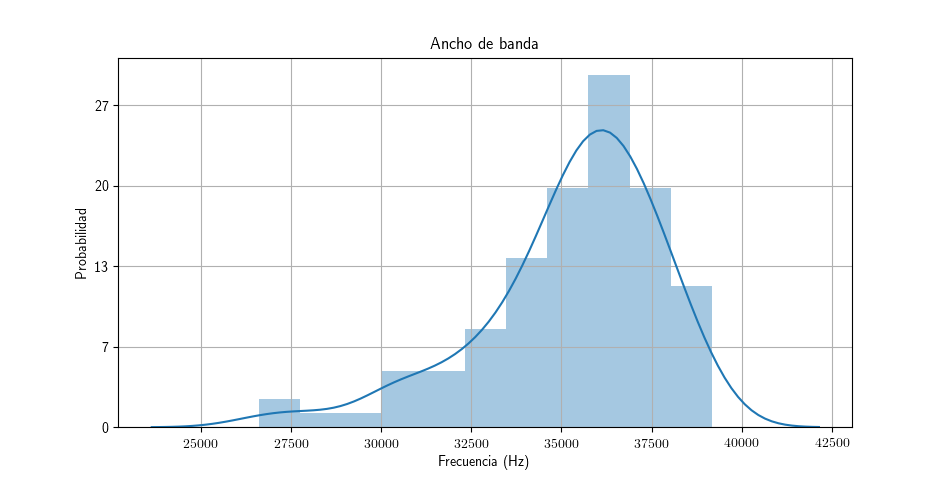
\includegraphics[scale=0.7]{imagenes/leg_hist_bw.png}
	\caption{Dispersi\'on de la frecuencia de corte del filtro 1}
\end{figure}

Se observa aqu\'i que si bien casi el 90\% de las curvas tienen $f_p \geq 33kHz$, existe la posibilidad de que esto no ocurra. Puesto que las tolerancias de los componentes no pueden mejorarse y todas las resistencias de una misma celda tienen el mismo valor y por lo tanto m\'inima sensibilidad a $Q$, se coloc\'o un preset en la $R_2$ de la \'ultima celda. Para peque\~nas variaciones de este valor alrededor de $R_1$, la variaci\'on de $Q$ deber\'ia ser pr\'acticamente nula, con lo cual se podr\'ia mover la frecuencia de corte del polo sin afectar el resto de los par\'ametros de la celda. Se verific\'o en \textit{Spice} que colocando un preset de $5k\Omega$ se podr\'ia mover la curva de la funci\'on transferencia al punto deseado.


\subsection{An\'alisis de resultados}

\begin{figure}[H]
	\centering
	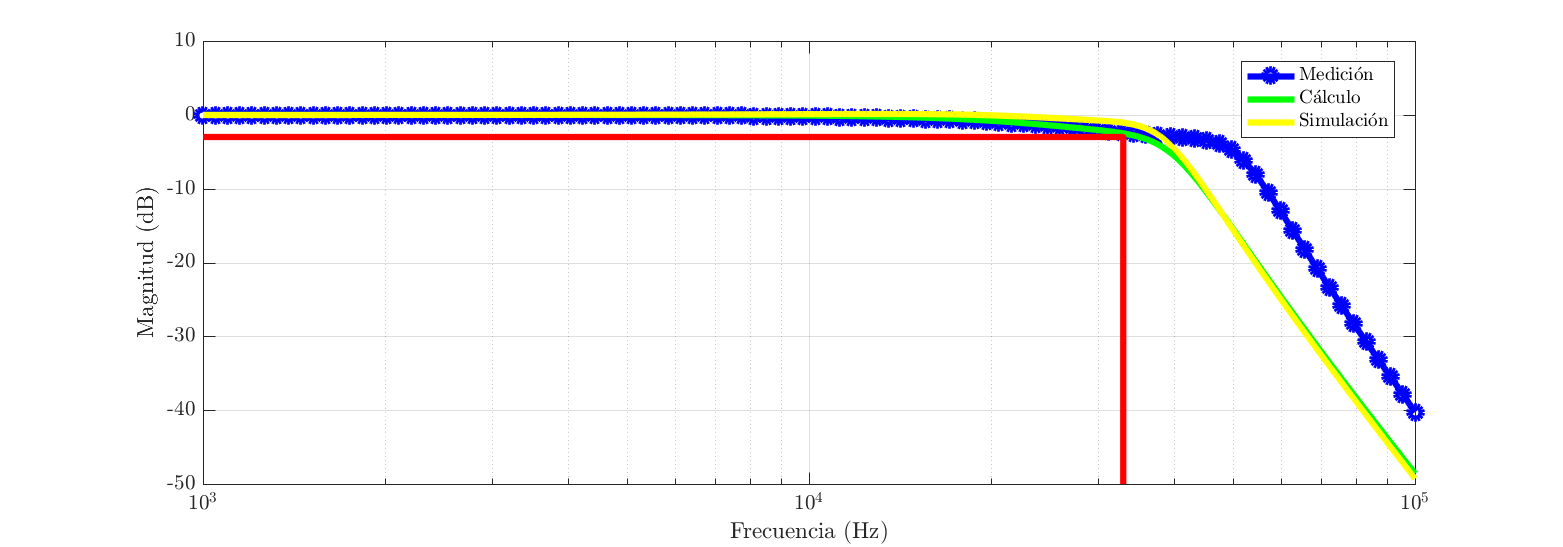
\includegraphics[scale=0.7]{imagenes/tc_tp5_ej1_leg_mag.png}
	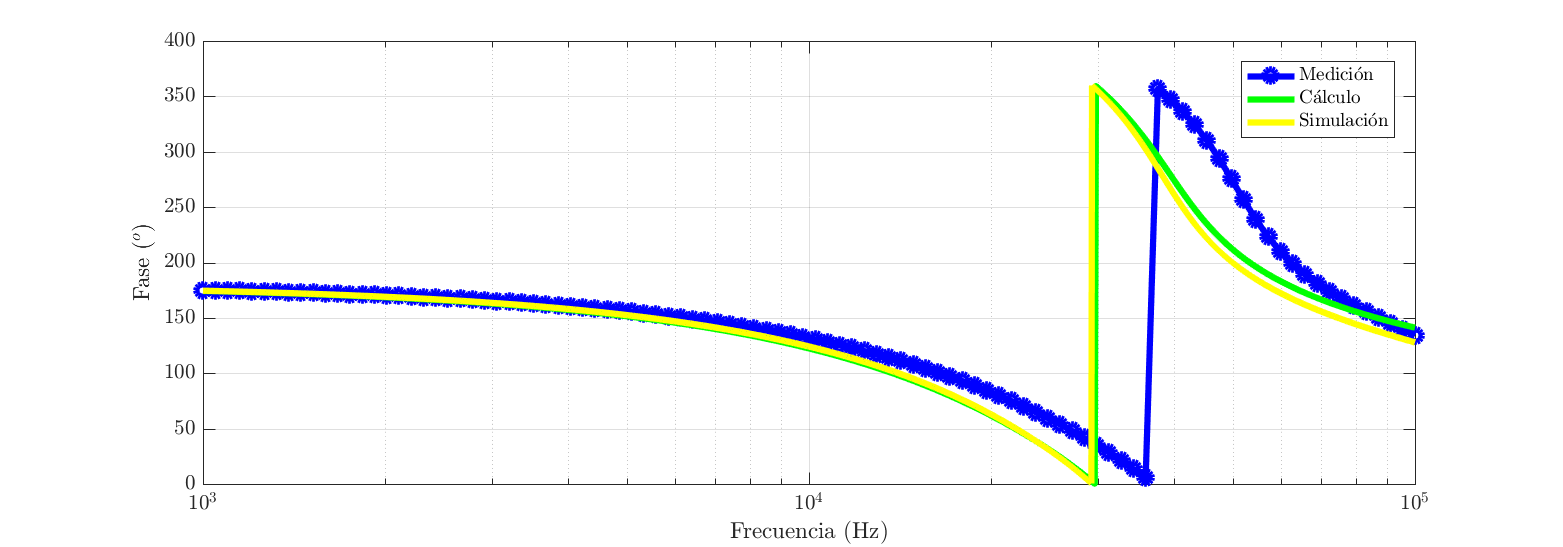
\includegraphics[scale=0.7]{imagenes/tc_tp5_ej1_leg_fase.png}
	\caption{Respuesta en frecuencia del filtro 1 (plantilla en rojo)}
\end{figure}

\begin{figure}[H]
	\centering
	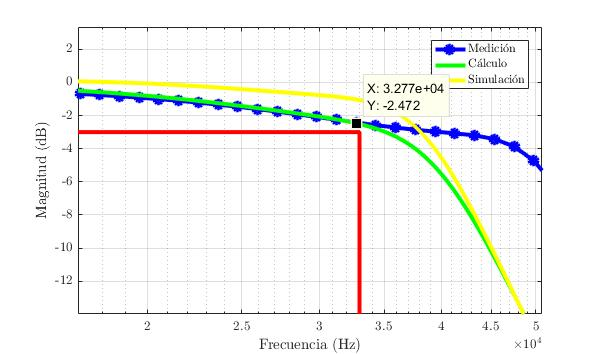
\includegraphics[scale=0.5]{imagenes/leg_bandapasante.jpg}
	\caption{Verificaci\'on de que el filtro 1 cumple con la plantilla propuesta}
\end{figure}

El circuito cumple satisfactoriamente con la plantilla propuesta. La forma de la respuesta en frecuencia del circuito coincide con la simulada y la calculada, pero la frecuencia de corte est\'a corrida aproximadamente $10kHz$. Esto puede deberse al ajuste que se tuvo que realizar con el preset: si la curva estaba corrida desde un principio por la dispersi\'on de los componentes (principalmente de los capacitores), al ajustar esa curva a una que cumpliera plantilla se puede haber obtenido un circuito considerablemente distinto al utilizado en la simulaci\'on. 

\section{Filtro 2: Bessel para baja se\~nal}

A continuaci\'on se implementar\'a un filtro con plantilla tanto de atenuaci\'on como de retardo de grupo. Para esto se utilizar\'a la aproximaci\'on de Bessel, y la tranferencia elegida se realizar\'a nuevamente con celdas Sallen-Key.

\begin{table}[H]
\centering
\begin{tabular}{|c|c|c|c|c|c|}
\hline
$f_p$    & $f_a$     & $A_p$ & $A_a$  & $\Upsilon(f_p)$ & $\abs{Z_{in}(f)}$            \\ \hline
$2200Hz$ & $10400Hz$ & $dB$  & $40dB$ & $\leq 5\%$    & $\geq 50k\Omega\, \forall f$ \\ \hline
\end{tabular}
\caption{Plantilla del filtro pasabajos con Bessel}
\end{table}

Al contrario del caso anterior, como tenemos un valor que cumplir de $A_a$ no se puede reducir libremente $A_p$ para tener mayor margen de error. En principio un filtro de grado 5 puede cumplir con la plantilla propuesta, pero se fracas\'o en intentos de obtener un Montecarlo satisfactorio para esta plantilla. Puesto adem\'as que la diferencia de complejidad entre un filtro de grado 6 con uno de grado 5 no es muy significativa utilizando estas celdas, dado que se utiliza la misma cantidad de operacionales y s\'olo se agrega un componente respecto del integrador compensado utlizado en el filtro anterior, se decidi\'o realizar tres etapas de segundo orden. \par 

Tambi\'en se verific\'o que esta la condici\'on de atenuaci\'on es mucho m\'as restrictiva que la de retardo de grupo, que en todos los casos probados se cumpl\'ia para frecuencias m\'as del doble de $f_p$ para filtros de grado 5 o 6 centrados en esta frecuencia. \par

Nuevamente, se armaron las etapas imponiendo la condici\'on de ganancia unitaria para todas ellas.

\begin{table}[H]
\centering
\begin{tabular}{|c||c|c|c|}
\hline
Etapa & Orden & $f_0\, (kHz)$ & Q    \\ \hline\hline
1     & 2     & 5.1           & 1.02 \\ \hline
2     & 2     & 4.3           & 0.61 \\ \hline
3     & 2     & 4.5           & 0.51 \\ \hline
\end{tabular}
\caption{Etapas del filtro 2}
\end{table}

En este caso, el criterio para ordenar las etapas fue el opuesto al anterior: como se especifica que este filtro es para bajas se\~nales, se procura que la amplificaci\'on en los sobrepicos tome lugar antes de la atenuaci\'on. \par

Los componentes se eligieron de la siguiente manera:

\begin{table}[H]
	\centering
\begin{tabular}{|c||c|c|c|c|}
\hline
Etapa & $R_1\, (k\Omega)$ & $R_2\, (k\Omega)$ & $C_1\, (nF)$ & $C_2\, (nF)$ \\ \hline\hline
1     & 1.00              & 1.00              & 63.7         & 15.2         \\ \hline
2     & 18.1              & 18.1              & 2.1          & 2.0          \\ \hline
3     & 1.00              & 1.00              & 42.9         & 28.7         \\ \hline
\end{tabular}
\caption{Valores de los componentes del filtro 2}
\end{table}

Nuevamente ocurre que con estos valores no se cumple la condici\'on de la plantilla para la impedancia de entrada. Considerando el circuito \ref{fig:1-celda}, se puede observar que cuando la frecuencia es lo suficientemente alta como para considerar despreciable a la impedancia de los capacitores, la impedancia de entrada de la celda es $R_1$: $V^+$ est\'a conectado a \textit{ground}, y $V^-$ a $V_{out}$, que a su vez est\'a conectado al nodo que se encuentra entre $R_1$ y $R_2$, y por lo tanto la tensi\'on despu\'es de $R_1$ es la de tierra y esta resistencia es el valor final de la impedancia de entrada. Sin embargo, si se buscan valores m\'as grandes de $R_1$ se comprometen la sensibilidad del factor de calidad de la celda a las resistencias, y adem\'as se obtienen valores de capacitores demasiado peque\~nos para resultar pr\'acticos.  Por lo tanto, se volvi\'o a utilizar un \textit{buffer} en la entrada, haciendo uso del operacional restante del integrado.\par 

Con tolerancias del 1\% para las resistencias y de 10\% para los capacitores, y utilizando nuevamente el TL074, se obtuvo la dispersi\'on de $f_p$ y de $f_a$ mediante un an\'alisis de Montecarlo con 100 curvas. 

\begin{figure}[H]
	\centering
	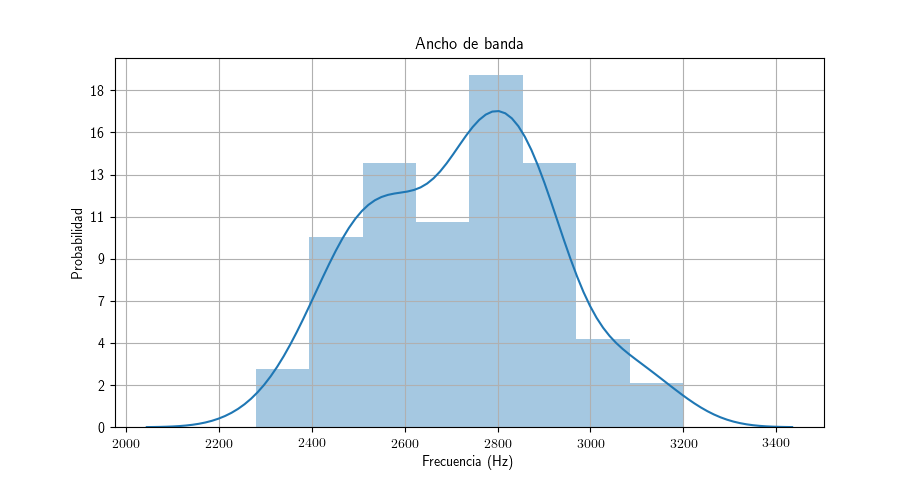
\includegraphics[scale=0.7]{imagenes/bes_hist_bw.png}
	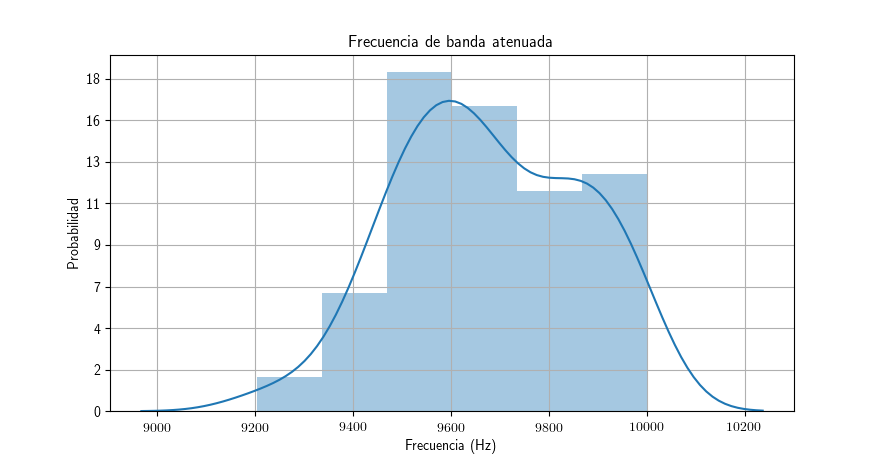
\includegraphics[scale=0.7]{imagenes/bes_hist_fa.png}
	\caption{Dispersi\'on de las frecuencia de corte y de atenuaci\'on del filtro 2}
\end{figure}

En principio la plantilla se cumple para todas las combinaciones calculadas de variaciones en los valores de los componentes respecto al nominal. Sin embargo, puesto que en ambos casos se est\'a en valores muy cercanos al de $f_p$ y $f_a$ de la plantilla en el peor caso, se coloc\'o un preset en la $R_2$ de la etapa 3 de todas maneras, a fin de potencialmente poder contrarrestar los efectos de factores no considerados en la simulaci\'on que terminen de correr la curva para la zona no aceptada. \par


\subsection{An\'alisis de resultados}

\begin{figure}[H]
	\centering
	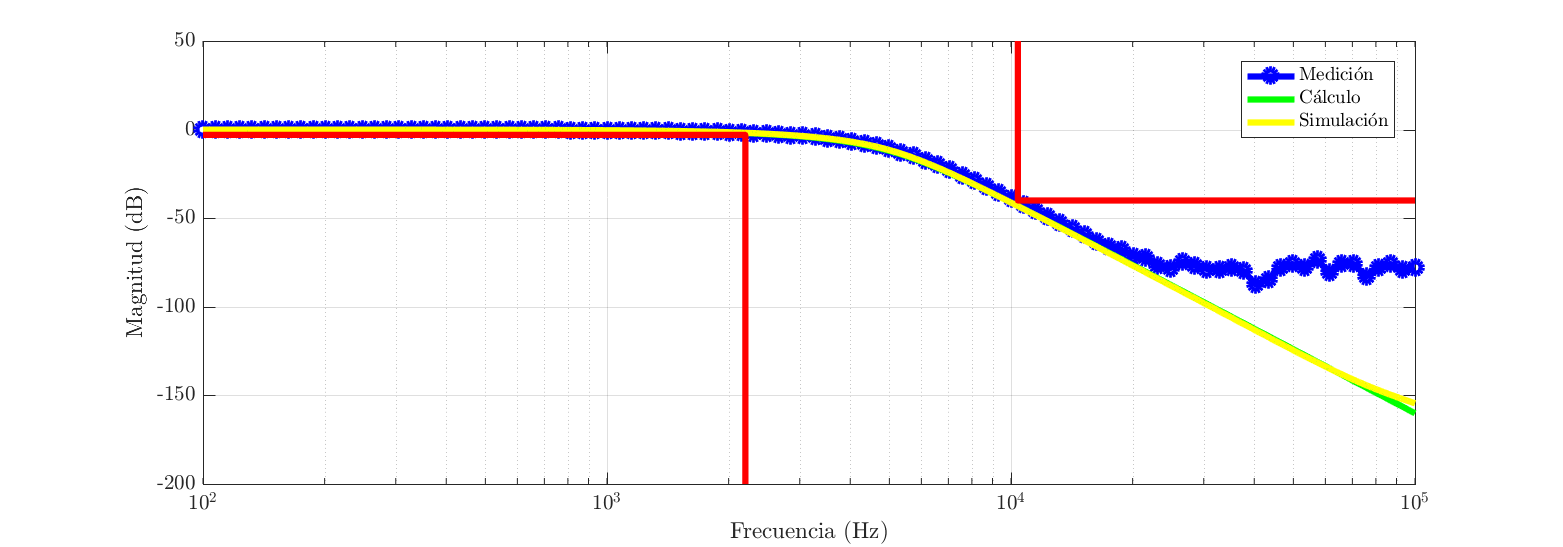
\includegraphics[scale=0.7]{imagenes/tc_tp5_ej1_bes_mag.png}
	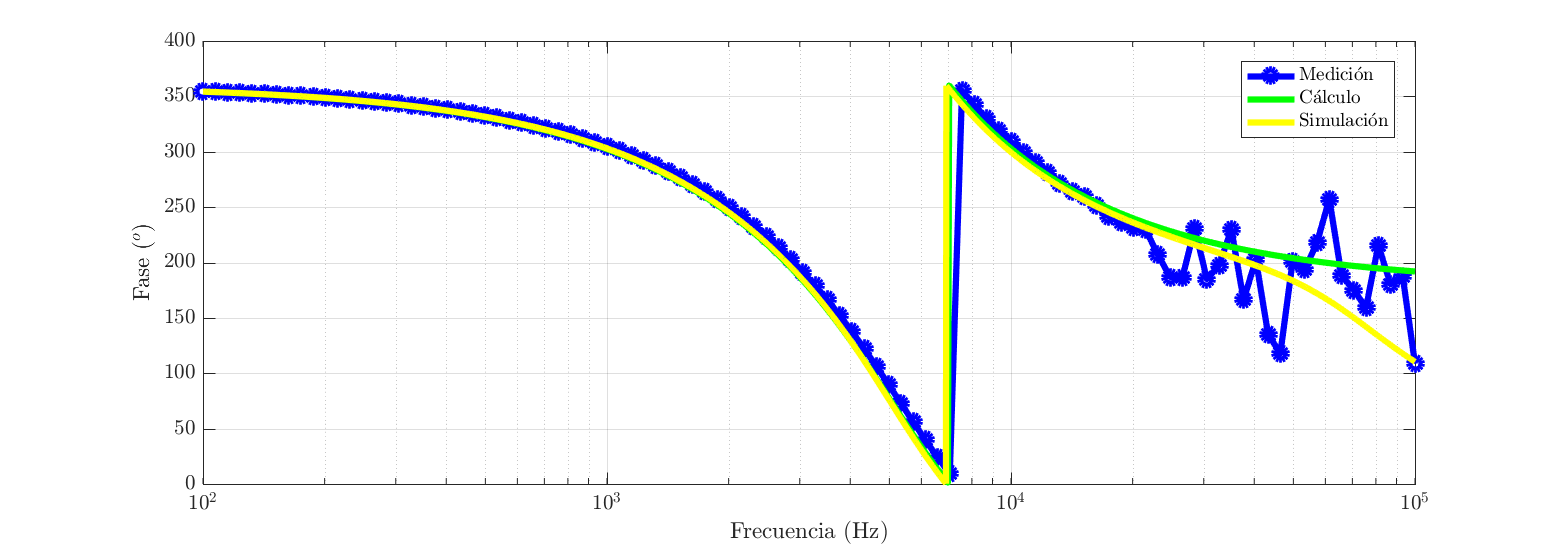
\includegraphics[scale=0.7]{imagenes/tc_tp5_ej1_bes_fase.png}
	\caption{Respuesta en frecuencia del filtro 2 (plantilla en rojo)}
\end{figure}


\begin{figure}[H]
	\centering
	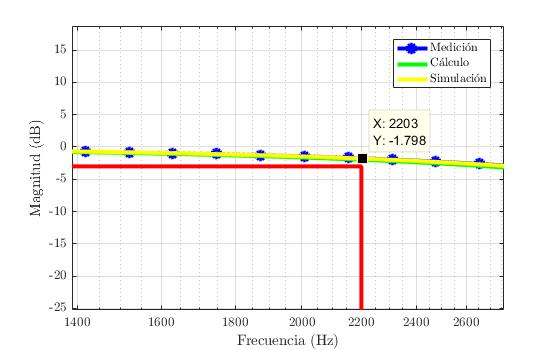
\includegraphics[scale=0.42]{imagenes/bes_bandapasante.jpg}
	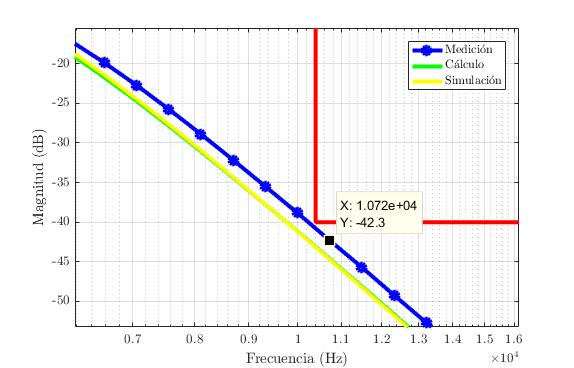
\includegraphics[scale=0.4]{imagenes/bes_bandaatenuada.jpg}
	\caption{Verificaci\'on de que el filtro 2 cumple con la plantilla de atenuaci\'on propuesta}
\end{figure}

El filtro se ajusta satisfactoriamente a la plantilla de atenuaci\'on., y su comportamiento es el mismo que el predicho por la simulaci\'on y los c\'alculos hasta frecuencias de $11kHz$. M\'as all\'a de eso no se pudo medir satisfactoriamente, puesto que la atenuaci\'on es demasiado grande como para obtener un valor representativo de la tensi\'on de salida. \par

Para comprobar que se cumple tambi\'en la plantilla de retardo de grupo, se calcul\'o num\'ericamente la derivada de la fase a partir de las mediciones obtenidas, y se determin\'o $\tau(0)$ como la primera de estas derivadas. 

\begin{figure}[H]
	\centering
	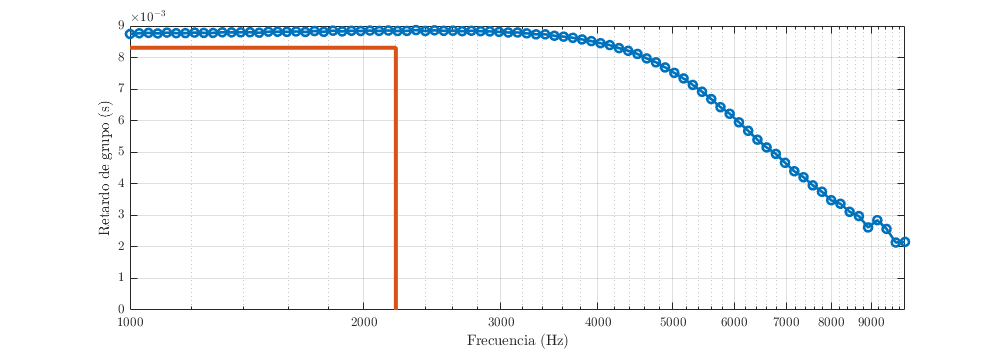
\includegraphics[scale=0.7]{imagenes/tc_tp5_ej1_gd.png}
	\caption{Retardo de grupo del filtro 2}
\end{figure}

De acuerdo a lo determinado en la simulaci\'on, a pesar de que la plantilla de simulaci\'on se cumple de forma ajustada, el retardo de grupo se mantiene dentro de la plantilla hasta aproximadamente $4000Hz$. Por lo tanto este filtro cumple la condici\'on impuesta para el retardo de grupo en $2200Hz$.

\section{Conclusiones}

Se lograron implementar dos filtros pasabajos con celdas Sallen-Key, de orden 5 y 6 respectivamente. El filtro de grado 6, calculado a partir de la aproximaci\'on de Bessel, exhibi\'o un comportamiento mucho m\'as similar al esperado que el de Legendre. Para este \'ultimo filtro tambi\'en se observ\'o una mayor dispersi\'on en $f_p$. Esto se puede deber a que en este filtro hab\'ia una etapa con las resistencias distintas entre s\'i, lo cual aumenta la sensibilidad de $Q$ a variaciones en los valores de los componentes. A su vez, los factores de calidad de las etapas de segundo orden del filtro realizado con Legendre eran m\'as altos que las de Bessel, con lo cual esta sensibilidad podr\'ia ser m\'as cr\'itica al afectar la frecuencia donde cae el sobrepico de la etapa. \par

Un problema que con certeza puede atribuirse al $Q$ elevado es la dificultad de encontrar componentes de valores razonables que se ajusten a las frecuencias de corte y factores de calidad pedidos. En la segunda etapa del filtro de Legendre, result\'o problem\'atico implementar un $Q$ de 2.23: se debi\'o usar un capacitor de $820pF$, que est\'a entre los \'ultimos valores que podr\'ia ser razonable usar en un circuito de estas caracter\'isticas. Para valores de $Q$ mayores problemente ser\'ia m\'as conveniente recurrir a otro tipo de celda. \par

De haber sido necesario implementar un $Q$ mayor con una celda Sallen-Key, se podr\'ia haber abandonado la simplificaci\'on de ganancia unitaria, puesto que para ganancias m\'as altas el factor de calidad aumenta en este circuito. Sin embargo, para este caso result\'o conveniente tener menos variables en juego a la hora de elegir los componentes. \par

\end{document}
